% 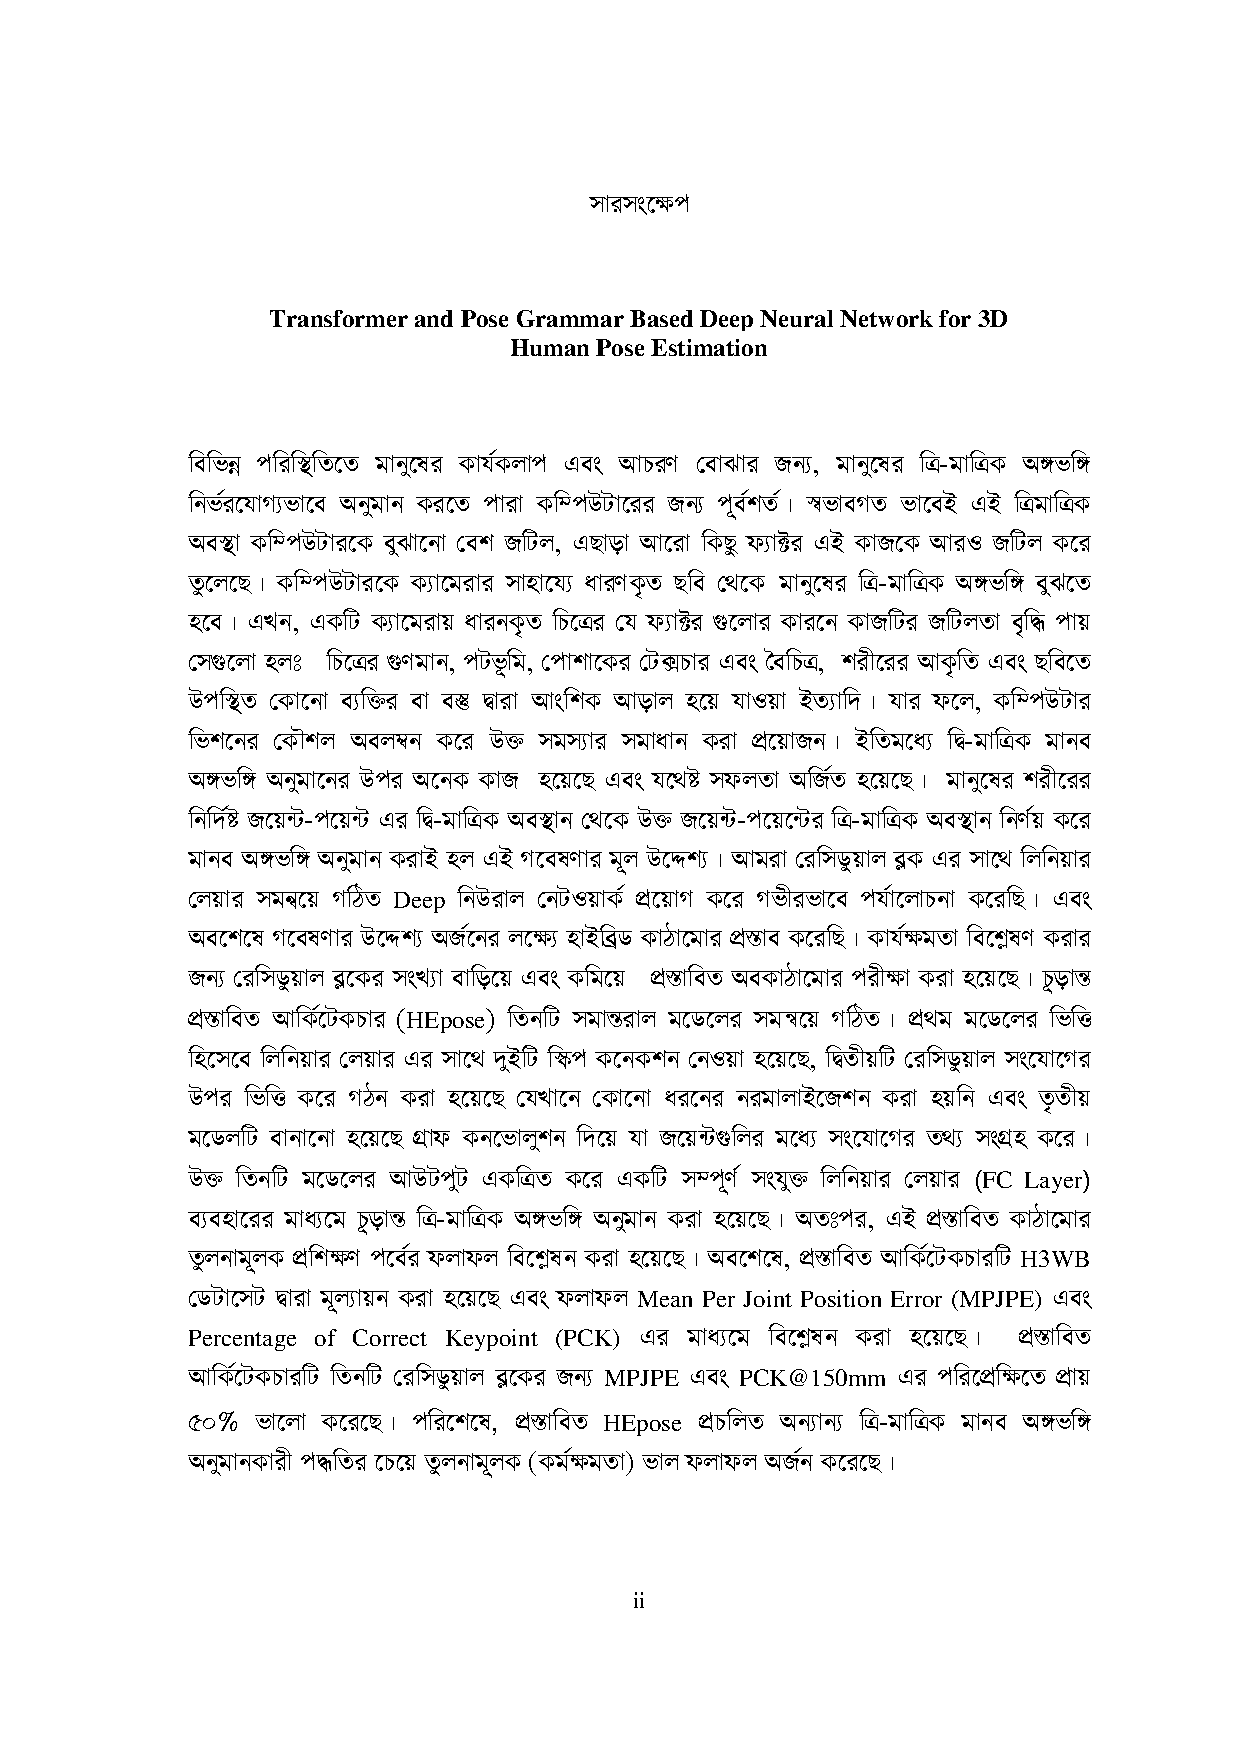
\includepdf[fitpaper=true, pages=-]{Appendix/abstract_bangla.pdf}

\doublespacing
\begin{center}
    \Large সারসংক্ষেপ\\
    \addcontentsline{toc}{chapter}{সারসংক্ষেপ}
    \singlespacing
    {\large\thesistitle}\\
\end{center}

ডিজিটাল নথি যাচাইকরণ প্রক্রিয়াকে আরও স্বচ্ছ ও নির্ভরযোগ্য করার জন্য একটি কাঠামো তৈরি করা হয়েছে। এই কাঠামোটি কৃত্রিম বুদ্ধিমত্তা এবং ব্লকচেইন প্রযুক্তির সমন্বয়ে গঠিত। প্রচলিত নথি যাচাইকরণ পদ্ধতিগুলোতে কিছু সীমাবদ্ধতা রয়েছে। এগুলো সাধারণত নির্দিষ্ট কর্তৃপক্ষের ওপর নির্ভরশীল এবং তারা যাচাইয়ের সিদ্ধান্ত নেওয়ার কোনো ব্যাখ্যা প্রদান করে না। ফলে অনেক সময় ভুল নথি গৃহীত হতে পারে এবং নথির প্রকৃত উৎস সম্পর্কে আমরা নিশ্চিত হতে পারি না। প্রস্তাবিত এই কাঠামোটি প্রধানত দুটি অংশে বিভক্ত। প্রথম অংশটি এমন একটি পদ্ধতি যা নথিগুলো বিশ্লেষণ করে তার পাঠ্য বা বিষয়বস্তু বুঝতে পারে; এটি পরীক্ষা করে দেখে যে শব্দগুলো মানুষের দ্বারা লিখিত নাকি কোনো কৃত্রিম বুদ্ধিমত্তা দ্বারা তৈরি এবং সেই অনুযায়ী নথিটি আসল না জাল তা নির্ধারণ করে। দ্বিতীয় অংশটি হলো একটি কার্যক্রম বা ‘স্মার্ট কন্ট্রাক্ট’, যা যাচাইকৃত নথিগুলোর রেকর্ড সংরক্ষণ করে। এই রেকর্ডটি ব্লকচেইনে রাখা হয় বলে এটি কখনোই পরিবর্তন বা জালিয়াতি করা সম্ভব নয়। এই সিস্টেমে ব্যবহারকারীদের জন্য নথি আপলোড এবং সেগুলো যাচাই করার সুব্যবস্থা রয়েছে। এটি এমনভাবে নকশা করা হয়েছে যাতে একসাথে অনেক নথির তথ্য একটি উপাদানসংগ্রহ সুশৃঙ্খলভাবে সংরক্ষণ করা যায়। আমরা যখন কিছু নমুনা নথির মাধ্যমে এই কাঠামোটি পরীক্ষা করেছি, তখন এটি অত্যন্ত সফলভাবে সদৃশ নথি এবং তৈরির উৎস সংক্রান্ত অসঙ্গতিগুলো শনাক্ত করতে সক্ষম হয়েছে। এই কাঠামোটির একটি বড় সুবিধা হলো এটি ব্লকচেইনের ওপর অতিরিক্ত তথ্যের চাপ সৃষ্টি করে না, যা একে বাস্তব ক্ষেত্রে ব্যবহারের উপযোগী করে তুলেছে। পরিশেষে বলা যায়, এই কাঠামোটি অত্যন্ত গুরুত্বপূর্ণ কারণ এটি প্রমাণ করে যে ডিজিটাল নথির সত্যতা নিশ্চিত করতে এবং মানুষের আস্থা অর্জনে কৃত্রিম বুদ্ধিমত্তা ও ব্লকচেইন প্রযুক্তিকে কার্যকরভাবে একসাথে ব্যবহার করা সম্ভব। এটি একটি বাস্তবমুখী সমাধান যা ডিজিটাল নথি সংশ্লিষ্ট বিভিন্ন পেশাদার ক্ষেত্রে অত্যন্ত কার্যকর ভূমিকা রাখতে পারে। ব্যাখ্যাযোগ্য কৃত্রিম বুদ্ধিমত্তা এবং ব্লকচেইনের এই সম্মিলিত ব্যবহার ডিজিটাল নথি যাচাইকরণকে আরও স্বচ্ছ, আধুনিক এবং শক্তিশালী করে তুলেছে।
